\documentclass[a4paper]{article}
\usepackage{graphicx}
\usepackage{xcolor}
\usepackage{url}
\usepackage{outlines}
\usepackage{listings}
\usepackage{fontspec}
\setmainfont{Calibri}
\lstset{basicstyle=\ttfamily,
	showstringspaces=false,
	commentstyle=\color{blue},
	keywordstyle=\color{pink}
}
\lstset{emph={
	nc,tcp,udp,http,},emphstyle=\color{purple}
}
\newcommand{\abc}{\hfill \break}
\usepackage{fancyhdr}
\usepackage{geometry}
\geometry{
	a4paper,
	total={170mm,257mm},
	left=20mm,
	top=20mm,
	bottom=39mm,
}

\setlength{\headheight}{82.70538pt}

\fancypagestyle{oida}{
	\fancyhf{}
	\fancyhead[L]{\fontsize{7.5}{7.5}htl donaustadt\\ Donaustadtstraße 45\\
		1220 Wien\\~\\ Abteilung: Informationstechnologie\\ 
	Schwerpunkt: Netzwerktechnik}
	\fancyhead[R]{
\includegraphics[scale=0.45]{images/logo.png}}

	\fancyfoot[L]{\today}
	\fancyfoot[C]{\jobname}
	\fancyfoot[R]{Seite: \thepage}
}

\begin{document}
\bibliographystyle{plain}
\pagestyle{oida}
\section*{Thema}
\par\noindent\rule{\textwidth}{0.4pt}

Laborprotokoll
Template

\begin{figure}[h]
	
\includegraphics[scale=0.3]{images/mika.jpeg}
	\caption{Wunderbares Gruppenlogo}
\end{figure}

\vspace*{\fill}
Unterrichtsgegenstand:	NWT|ZIVK

Jahrgang:	3AHITN

Name:	Stefan Fürst, Marcel Raichle

Gruppenname/Nummer: Dumm und Dümmer/7

Betreuer: 	ZIVK/ANGE

Übungsdaten:

Abgabedatum:


\newpage
\tableofcontents

\newpage

\section{Aufgabenstellung}



\section{Zusammenfassung}

\newpage

\section{Vollständige Netzwerktopologie der gesamten Übung}

\newpage

\section{Übungsdurchführung}
\subsection{Configure the router}

\subsection{Configure Devices and Verify Connectivity}
\subsubsection{Configure the PC interfaces}

\begin{figure}[h]
	\centering
	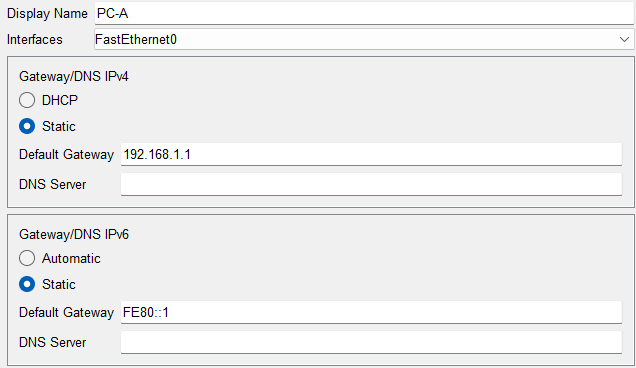
\includegraphics[scale=0.3]{images/pc-a-gateway.png}
	\caption{PC-A Gateway-config}
\end{figure}
\begin{figure}[h]
	\centering
	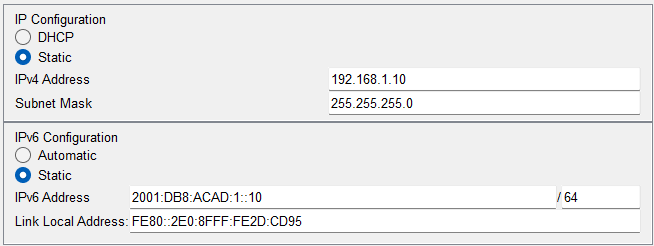
\includegraphics[scale=0.3]{images/pc-a-fa.png}
	\caption{PC-A Interface-confing}
\end{figure}
\begin{figure}[h]
	\centering
	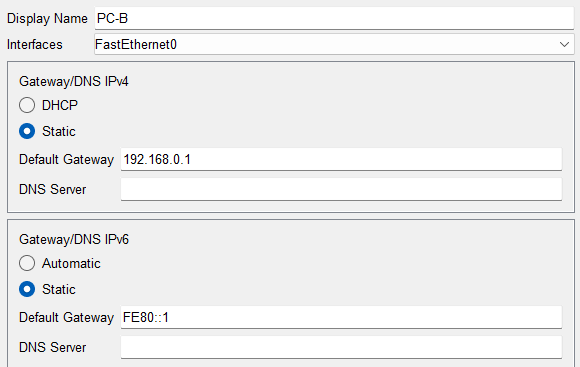
\includegraphics[scale=0.3]{images/pb-b-gateway.png}
	\caption{PC-B Gateway-config}
\end{figure}
\begin{figure}[h]
	\centering
	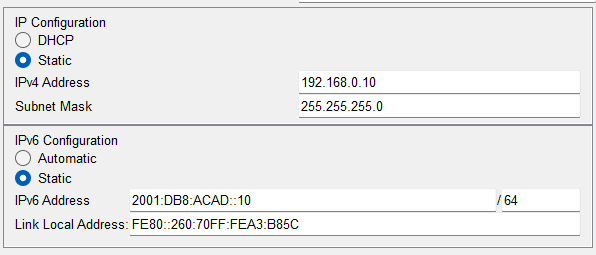
\includegraphics[scale=0.3]{images/pc-b-fa.png}
	\caption{PC-B Interface-confing}
\end{figure}

\subsection{Verify network connectivity}
\begin{figure}[h]
	\centering
	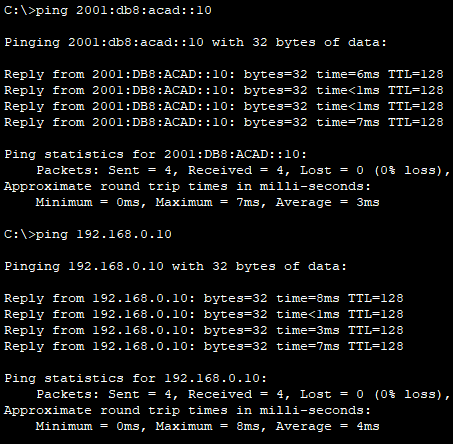
\includegraphics[scale=0.3]{images/ping.png}
	\caption{Pinging PC-B from PC-A}
\end{figure}
\subsubsection{Connecting to the Router with ssh}


\subsection{}
\section{Vollständige Konfigurationsdateien}

\newpage

\section{Quellen}
\bibliography{quellen}
\newpage
\section{Abbildungsverzeichnis}

\listoffigures

\end{document}
